\documentclass[letterpaper]{article}
\usepackage[english]{babel}
\usepackage[utf8]{inputenc}
\usepackage{amsmath}
\usepackage{listings}
\usepackage{graphicx}
\usepackage{hyperref}

\title{Big Data Project Report}
\author{Shenwei Liao, Anthony Ou, Jacqueline Terlaan\\
	CMPUT 391\\
Winter 2014}

\begin{document}
\maketitle
\section{Introduction to Cassandra}
\lstset{postbreak=\space, breakindent=5pt, breaklines}

\subsection{What is NoSQL?}
NoSQL is a term that describes any database system which does not strictly
conform to the relational database model. We may have any one of the
following:
\begin{itemize}
	\item Does not meet all "ACID" properties.
	\item May store data in a fashion other than a strictly
		relational set of tables.
\end{itemize}

\subsection{Why NoSQL?}
\begin{itemize}
	\item We have some BIG data to deal with (several TB), and growing!
	\item Big Data implies distribution;
	\item Distribution implies CAP theorem;
	\item CAP theorem implies compromises!
\end{itemize}

\subsection{What is Apache Project's Cassandra?}
Apache Cassandra is an open-source NoSQL DBMS based on a
column-oriented data model. 
Features:
\begin{itemize}
	\item Available, Partition-tolerant
	\item Eventually consistent
	\item High scalability
	\item "Schemaless" (implicit schema)
	\item Has its own query language: Apache cql
	\item Data compaction
\end{itemize}

\subsection{Why Cassandra?}
\begin{itemize}
	\item Partition-tolerant (essential for clustered systems).
	\item Available: mirrors "real-world" constraints on call-detail record
		systems.
	\item Eventual consistency is an acceptable compromise; we are not
		running a mission-critical system (like a bank), and most of our
		data insertion is similar to logging data.
	\item Cassandra is especially well-suited to storing logs.
	\item Widely used and relatively bug-free, especially for such "new" 
		software.
	\item Handles map-reduce and low-level details of storage process for nodes,
		as well as performing maintenance (as specified by DB admin), such
		as compaction.
	\item Very low chance of data loss (except if the DBA makes a mistake),
		even when upgrading Cassandra.
\end{itemize}

\section{Goals and Objectives}
\begin{itemize}
	\item To successfully implement a distributed database system which
		will reliably store at least 16TB of random data consisting of
		random numbers and strings organized into large tables with
		many columns (attributes).
	\item To distribute the data in the above tables across 8 "nodes"
		(servers), which form our "cluster".
	\item To generate additional tables distributed throughout the cluster
		to be optimally configured for the queries to meet their own
		requirements (see below).

	\item To query the above tables such that all of the following requirements
		are met by five queries.
		\begin{enumerate}
			\item Four of five queries must retrieve data across from all of the distributed nodes.
			\item At least one of the queries must contain at least ten atomic
				conditions (formulas) in the WHERE clause.
			\item At least two of the queries must utilize both the GROUP BY and
				ORDER BY clauses. Since Cassandra does not yet support GROUP BY
				aggregation, the same functionality must be acheived in another
				way.
			\item At least three of the five queries must be range queries which
				specify an upper and lower bound on some ordered attribute that
				is used for the purposes of querying.
			\item None of the five queries can be trivial. That is, there can be
				no simple key searches or anything that is of little practical
				interest for measuring how a database system can deal with
				computationally expensive requests.
		\end{enumerate}

	\item To record the execution time of each query.
\end{itemize}

\section{Methodology, Tools and Equipment Used}
8 server instances were used, each with 32GB virtual memory and 1TB secondary storage 

\section{Implementation}

\section{Shell Script}
A shell script was written to wrap all functionality of the OLAP project,
including server setup for all nodes, table creation and population and
executing the queries. To run it, cd into the directory containing group3.sh,
and call sh group3.sh, and follow the prompts interactively.

\subsection{Configuration Changes}
Many different aspects of Cassandra cluster and the table were tuned so that we
can achieve a high write availability and high performance for generating
a randomly generated dataset. Here are some of the more notable configuration
changes that we applied:
\begin{itemize}
	\item Cluster-wide changes (in cassandra.yaml):
		\begin{enumerate}
			\item Use of RoundRobinScheduler over NoScheduler.
				Having a request scheduler allowed for requests
				to be assigned to nodes faster by the
				coordinating node, speeding up
				concurrent reads and writes.
			\item Reducing commit log sync frequency. Writing to
				the commit log must happen for every
				transaction, as is necessary for write
				durability. For the purposes of this project,
				we can sacrifice some durability to go faster.
			\item Concurrent writes increased.
			\item Memtable flush writers increased. Memtable is the
				in-memory data structure cassandra uses to hold
				batched writes.
			\item Disabling automatic backups and snapshots of the
				keyspace. 
			\item Removed the throttling on compaction throughput.

		\end{enumerate}
	\item Table-specific changes:
		\begin{enumerate}
			\item Replication factor set to 3.
			\item Durable writes are disabled. The commit log
				doesn't need to be written to just for table
				generation. This and the next setting are only
				off because we are randomly generating data and
				there isn't such a thing as a wrong random
				value.
			\item Consistency level for inserts was set to 0 for
				maximum write availability.
			\item Compression is disabled.
		\end{enumerate}
\end{itemize}

\subsection{Table Schemas}
The cdr table follows the assignment specification's schema, with 400 columns.
It 
and 10 column keys, indexed on MONTH\_DAY and MOBILE\_ID\_TYPE. QUERY3 shows the
performance 
The role of the last two
tables is to make the substitute
aggregate queries both possible (as Cassandra has no
explicit support for GROUP BY aggregation) and
efficient (preprocessing data to be optimal for
queries).
\begin{enumerate}
	\item "CDR"
		The large 400 column table (column family) with 10
		column keys and 1 partition key. This table is 

	\item "QUERY3"
		Contains the same data as cdr, but the column keys are
		ordered MSC\_CODE first in an attempt to optimize for
		range-queries based on values of those column keys.
	\item "GROUP\_BY\_MONTH" 
		\begin{itemize}
			\item Keys are between 1 and 31.
			\item Reduces data to facilitate completion of
				a query equivalent to one in SQL
				containing 'GROUP BY MONTH\_DAY'.
			\item Uses 'WITH CLUSTERING ORDER
				BY(MONTH\_DAY)' to facilitate ordering
				the resulting tables contents by the
				day of the month.  
		\end{itemize}
	\item "GROUP\_BY\_MOBILE\_ID\_TYPE"
		\begin{itemize}
			\item Keys are between 0 and 7.
			\item Similar to "GROUP\_BY\_MONTH", but instead
				the assignment of the rows' locations
				is based on its insertion number modulo
				8.
			\item 'CLUSTERING ORDER BY(MOBILE\_ID\_TYPE)'
				used to order the rows with respect to
				MOBILE\_ID\_TYPE instead of the aggregate
				group MONTH.
		\end{itemize}
\end{enumerate}

\subsection{Programs}
We wrote two main Python 2.7 scripts: generate.py and query.py.

generate.py generates data 
-generate.py
-Begins with attempting to establish a connection to the local machine which is part
of the cluster. Constructs a connection object called 'session'.
-Expects program arguments: 
-The number of days to generate data for. 
-Different seed values to prevent collisions of data insertions.
-Cassandra has no support for primary keys; collisions result in overwriting data.
-Allows for multiple concurrent instances of data generation.
-Without seed argument, the script will use its default seed value (typically used
for consistency in generation of data) and will drop all of the data before completely
regenerating it.
-Depending on the results from stat.py (see below), 
-Asynchronously executes the insertion statements 
-randword() function
-Accepts parameter 'length' (intended to be a positive, nonzero numeric type)
-Generates a random lowercase string which is 'length' characters long.
-generate() function
-Allows for custom ranges on specified columns.
-Allows for custom data for specified data types.

-stat.py (mainly for testing)
-Reads in the contents of "partial\_data\_table.txt" and
"cdr\_table.txt", then counts the number of non-empty columns for
each row.
-Prints the resulting number (frequency) of items for each column.



\subsection{CQL Queries}

\begin{enumerate}
	\item Query 1
		\lstinputlisting{queries/query1.sql}

		Cluster-wide range query with 10 atomic formulas. Searches on
		every column key of the CDR table, as this is the only
		conceivable way to properly execute a range query.  Returns
		results from each node, satisfies the range query requirement
		and has 10 atomic formulas.

		Potential uses: many 'outliers' are eliminated from the
		selection because they are above and below the minimum and
		maximum values of all the columns
		respectively, by approximately 10\%. In other words, any
		'extreme' data points in the CDR table can be ignored for
		statistical analysis.

		Query 1 ('Alternate')
		\lstinputlisting{queries/query1a.sql}

		Performs the same cluster-wide query as Query 1, but over the table cdr\_alt,
		which resides in the keyspace 'group3alt' instead of 'group3'.

		Potential uses: essentially the same as those for Query 1, but in cases
		where less information from each row is required to complete the query,
		or when query execution must be fast.

		Query 1 ('Small')
		\lstinputlisting{queries/query1s.sql}

		Performs the same cluster-wide query as Query 1, but over the table smallcdr,
		which resides in the keyspace 'group3alt' instead of 'group3'. This query
		is intended to take less time than the previous query, because fewer columns
		have to be read into memory in order for the atomic conditions to be evaluated.

		Potential uses: essentially the same as those for Query 1, but in cases
		where less information from each row is required to complete the query,
		or when query execution must be even faster than Query 1 'Alternate'.

	\item Query 2
		\lstinputlisting{queries/query2.sql}

		Satisfies two requirements: cluster-wide and range query. Retrieves the number of
		cdr entries for cities with IDs strictly greater than 5000 and strictly less than
		90000. Limits the maximal number of elements counted to 40000000. Filtering of
		results is enabled.

		Potential uses: In some cases companies may wish to know how many calls were made
		in a given range of cities, based on certain CITY\_IDs. While
		those cities may not have any major features in common, this
		query can be used in cases where only a small
		sample of all cities is required.

	\item Query 3
		\lstinputlisting{queries/query3.sql}

		Satsifies two requirements: cluster-wide and range query. Counts the number of cdr
		entries such that DUP\_SEQ\_NUM is strictly greater than 30000 and strictly less than
		300000. All other atomic conditions in the range query are used to ensure that
		all of the results fall within a valid range and have no null-valued entries for
		CITY\_ID, SERVICE\_NODE\_ID, and so on. Because we are trying to query mainly by 
		DUP\_SEQ\_NUM, we allow filtering on the query in order to speed up execution.

		Potential uses: Suppose that statistical data is to be generated for rows in the
		CDR table for which there are no null-valued entries in the columns CITY\_ID,
		SERVICE\_NODE\_ID, RUM\_DATA\_NUM, MONTH\_DAY and DUP\_SEQ\_NUM, and that DUP\_SEQ\_NUM
		falls within a more specific range, that is 30000-300000 (not inclusive). The
		records could then be analyzed and compared to data for which not all of the
		attributes above are null, to compare behaviors of callers with different amounts
		of privacy. This could address questions such as "do people with more privacy make
		certain types of calls compared to people who do not?".

	\item Query 4
		\lstinputlisting{queries/query4.sql}

		Satisfies two requirements: group-by and order-by clause, and cluster-wide query.

		A table of counters aggregates the keys of the MOBILE\_ID\_TYPE columns with the 
		count of each number of rows in the CDR table with matchine MOBILE\_ID\_TYPE.
		Ordering by mobile\_id\_type is acheived by using a the 'USE CLUSTERING ORDER' 
		clause in the data definition statement in generate.py.
		We then retrieve GROUP\_BY\_MOBILE\_ID\_TYPEs contents and the count of its rows
		in order of appearance, i.e., the order in which the aggregated rows are sorted.

		MOBILE\_ID is the insertion number modulo 8 (or however many nodes), therefore
		the rows of the MOBILE\_ID table are evenly distributed throughout the cluster.
		This means that we can easily use this query as a check for correctness of
		the insertion process, as counting the number of rows in the MOBILE\_ID\_TYPE table
		on each node should total up to the number of unique items in the database.

		This is an atomic, yet seemingly asynchronous transaction. In other words, only
		small critical sections of execution are protected for short amounts of time
		to prevent collisions, but otherwise parallelism is fully exploited (with minimal
		constraints of Ahmdal's Law) due to the very even distribution of data across all 
		8 nodes. 

		Updating counter columns is done in the following way:

		update group\_by\_MOBILE\_ID\_TYPE set count = count + 1  where MOBILE\_ID\_TYPE = ? and id = 1;

		Potential uses: Most likely for the generation of histograms, but other basic
		kinds of statistical analysis can be performed on these small MOBILE\_ID\_TYPE 
		'buckets' as well, such as calculating arithmetic averages, etc.

	\item Query 5
		\lstinputlisting{queries/query5.sql}

		Satisfies the group-by and order-by clause requirements. 
		'CLUSTERING ORDER BY (MONTH\_DAY)' ensures that the GROUP\_BY\_MONTHs entries are ordered
		by MONTH\_DAY, and GROUP BY functionality is acheived via aggregating the COUNT type
		column 'COUNTER' into MONTH\_DAY groupings. The resulting COUNTER column typically
		contains values which are quite close in value, but with some differences between
		them due to the pseudorandom generation and distribution of data.

		Potential uses: finding out which day(s) of each month of the year have the highest
		frequency of entries added to the CDR table can be of use for marketing to customers,
		optimizing billing rates, and so on. Similar queries can be written for different
		times of the day, months or weeks of the year, by aggregating CDR row counts into 
		hourly, monthly or weekly groupings for more specific results which could be of use 
		in billing plans with calls at different times incurring different costs.
\end{enumerate}

\section{Notes on GROUP BY Queries}
Recall that a GROUP BY aggregation is basically a function which
gathers rows of data retrieved by a query and groups them
together based on an attribute. Since cassandra doesn't support doing
GROUP BYs on the fly (a trade off to provide faster column-oriented reads and
writes, they are done at insert time, by creating tables with redundant,
sorted data.

\section{Experimental Results}

\subsection{Table Population}

A test cluster was used for some preliminary tests. With the
various configuration tweaks described above, insertion of about 300,000
entries --- resulting about 40GB of data per node --- took 35.5 minutes.
The biggest table to generate took two and a half days, generating an average
of 380GB per node for a total of just over 3TB of data, out of the 8TB that was
available on the cluster. The average speed of insertions to the big table was
roughly 15MB/s. 

\subsection{Query Results}

Our queries ran pretty quickly as expected. The GROUP BY queries predictably executed the
fastest, as the work was already done at insertion time.
\begin{figure}[h]
	\centering
	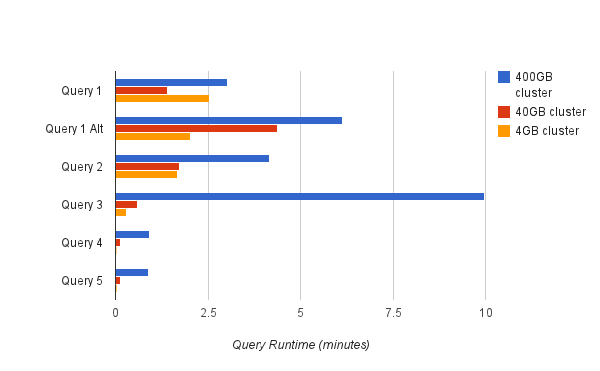
\includegraphics[resolution=300]{chart}
	\label{fig:Query Execution Times}
\end{figure}

\section{Discussion}

It was unclear why query 1 performed faster than query 2 even though query 1
has 6 more column keys and 200 fewer resulting rows. Another anomaly was that
removing column keys from query 1 did not improve performance as it was
hypothesized to.

\section{Conclusions}

The most important changes that affected insert speed was using the round
robin scheduler to have more nodes handle requests in parallel, and to disable
the commit log/durable writes in order to get more disk IO.

The queries on the other hand were pretty straightforward, except for the fact
that GROUP BYs have to be done a priori, as Cassandra has no facility to do
them on the fly.

\section{Notes on Possible Improvements}

Some tests were run on query 1 to assess the performance increase of data
partitioning. We weren't able to re-generate the large table to see the effects
on that, but trials on a smaller table reduced the runtime of query 1 from 2.6
minutes down to 1.0 minute. We haven't tested it on a larger scale, but would
say that it has lots of potential to speed up querying, without much hit to our
table populating speed.

\section{References Used}

Agilent Technologies Inc (28 October, 2014), "Mobile Station Reported Pilot Information".
\url{http://wireless.agilent.com/rfcomms/refdocs/cdma2k/c2kla_gen_ms_pilot_meas_report.html}
Accessed: 10 March 2014.

Apache Software Foundation (2004), "The Apache Licence, Version 2.0".
\url{http://www.apache.org/licences/LICENCE-2.0}
Accessed 7 March, 2014.

Apache Software Foundation (10 March 2014), "Cassandra Query Language (CQL) v3.1.5".
\url{http://cassandra.apache.org/doc/cql3/CQL.html}
Accessed: 10 March 2014.


Apache Software Foundation (15 November 2013), "UUID".
\url{http://wiki.apache.org/cassandra/UUID}
Accessed: 13 March 2014.


DataStax Documentation (2014), "Cassandra Storage Basics".
\url{http://www.datastax.com/documentation/cassandra/2.0/cassandra/dml/manage_dml_intro_c.html}
Accessed 7 March, 2014.

DataStax Documentation (2014), "The cassandra.yaml Configuration File".
\url{http://www.datastax.com/documentation/cassandra/2.0/cassandra/configuration/configCassandra_yaml_r.html}
Accessed 7 March, 2014.  

DataStax Documentation (2014), "CLI keyspace and table storage configuration".
\url{http://www.datastax.com/documentation/cassandra/2.0/cassandra/reference/referenceStorage_r.html}
Accessed: 10 March 2014.

DataStax Inc. (2014), "UUID and timeuuid".
\url{http://www.datastax.com/documentation/cql/3.0/cql/cql_reference/uuid_type_r.html}
Accessed: 13 March 2014.

DataStax Documentation (2014), "What's new in Cassandra 2.0".
\url{http://www.datastax.com/documentation/cassandra/2.0/cassandra/features/features_key_c.html}
Accessed: 10 March 2014.

DataStax Documentation (2014), "The Write Path to Compaction".
\url{http://www.datastax.com/documentation/cassandra/2.0/cassandra/dml/dml_write_path_c.html}
Accessed 7 March, 2014.


Fowler, M. (9 January 2012), "NosqlDefinition".
\url{http://martinfowler.com/bliki/NosqlDefinition.html}
Accessed: 13 March 2014.

Fowler, M. (16 November 2011), "PolyglotPersistence".
\url{http://martinfowler.com/bliki/PolyglotPersistence.html}
Accessed: 13 March 2014.

Fowler, M. (7 January 2013), "Schemaless Data Structures".
\url{http://martinfowler.com/tags/noSQL.html}
Accessed: 14 March 2014.


Grinev, M. (9 July 2010), "A Quick Introduction to the Cassandra Data Model".
\url{http://maxgrinev.com/2010/07/09/a-quick-introduction-to-the-cassandra-data-model/}
Accessed: 10 March 2014.

Grinev, M. (12 July 2010), "Do You Really Need SQL to Do It All in Cassandra?".
\url{ http://maxgrinev.com/2010/07/12/do-you-really-need-sql-to-do-it-all-in-cassandra/}
Accessed: 10 March 2014.


McFadin, P. (13 November 2012), "Cassandra Data Modeling Talk".
\url{http://www.slideshare.net/patrickmcfadin/data-modeling-talk}
Accessed: 13 March 2014.

McFadin, P. (3 May 2013), "The Data Model is Dead, Long Live the Data Model!".
\url{http://www.slideshare.net/patrickmcfadin/the-data-model-is-dead-long-live-the-data-model}
Accessed: 14 March 2014.

McFadin, P. (16 May 2013), "Become a Super Modeler".
\url{http://www.slideshare.net/patrickmcfadin/become-a-super-modeler}
Accessed: 14 March 2014.

McFadin, P. (24 June 2013), "The World's Next Top Data Model".
\url{http://www.slideshare.net/patrickmcfadin/the-worlds-next-top-data-model}
Accessed: 14 March 2014.

McFadin, P. (11 October 2013), "Cassandra 2.0: Better, Stronger Faster".
\url{http://blog.imaginea.com/consistency-tuning-in-cassandra/}
Accessed: 14 March 2014.

McFadin, P. (17 February 2014), "Time Series with Apache Cassandra".
\url{http://www.slideshare.net/patrickmcfadin/time-series-with-apache-cassandra-strata}
Accessed: 13 March 2014.

Oracle Inc. (Copyright 1996-2005), "Datatype Comparison Rules".
\url{http://docs.oracle.com/cd/B19306_01/server.102/b14200/sql_elements002.htm#i55214}
Accessed: 10 March 2014.

Oracle Inc (No date), "GROUP BY clause".
\url{http://docs.oracle.com/javadb/10.6.1.0/ref/rrefsqlj32654.html}
Accessed 7 March, 2014.

Oracle Inc (No date), "ORDER BY clause".
\url{http://docs.oracle.com/javadb/10.6.1.0/ref/rrefsqlj13658.html}
Accessed: 10 March 2014.

Oracle Inc (No date), "SelectExpression".
\url{http://docs.oracle.com/javadb/10.6.1.0/ref/rrefselectexpression.html#rrefselectexpression}
Accessed: 10 March 2014.

Oracle Inc. (Copyright 1996-2005), "SYSDATE".
\url{http://docs.oracle.com/cd/B19306_01/server.102/b14200/functions172.htm}
Accessed: 10 March 2014.

Oracle Inc. (Copyright 1996-2005), "SYSTIMESTAMP".
\url{http://docs.oracle.com/cd/B19306_01/server.102/b14200/functions173.htm}
Accessed: 10 March 2014.

Oracle Inc. (Copyright 1996-2005), "TO\_DATE".
\url{http://docs.oracle.com/cd/B19306_01/server.102/b14200/functions183.htm}
Accessed: 10 March 2014.

Saxena, S. (4 September 2013), "Consistency Tuning In Cassandra".
\url{http://blog.imaginea.com/consistency-tuning-in-cassandra/}
Accessed: 14 March 2014.


\end{document}
